\documentclass[a4paper,12pt]{report}

% Language setting
% Replace `english' with e.g. `spanish' to change the document language
\usepackage[english]{babel}

% Set page size and margins
% Replace `letterpaper' with`a4paper' for UK/EU standard size
\usepackage[a4paper,top=2cm,bottom=2cm,left=2cm,right=2cm,marginparwidth=1.75cm]{geometry}

% Useful packages
\usepackage{algorithmic}
\usepackage{amsmath}
\usepackage{graphicx}
\usepackage{listings} 
\usepackage{color}
\usepackage{xcolor}
\usepackage{hyperref}
\usepackage{verbatim}
\usepackage{adjustbox}
\usepackage{svg}
%Tudor Add-ons
\usepackage[bottom]{footmisc}
\usepackage[nottoc]{tocbibind}
\usepackage{geometry}
\usepackage{capt-of}
\usepackage{tabularx}
\usepackage{calc}
\usepackage{tcolorbox}
\usepackage[T1]{fontenc}
\usepackage{lmodern} %font for vhdl listings

\tcbuselibrary{breakable}
\setcounter{tocdepth}{3}
\setcounter{secnumdepth}{3}

\definecolor{remark-golden}{RGB}{255,220,115}
\definecolor{list-turqoise}{RGB}{56, 119, 128}
\definecolor{table-blue}{RGB}{15, 87, 168}
\definecolor{listing-purple}{RGB}{110, 28, 122}
\definecolor{vhdl-fuchsia}{RGB}{128, 0, 128}
\definecolor{vhdl-green}{RGB}{17, 107, 7}
\definecolor{vhdl-tag-green}{RGB}{40, 166, 12}
\definecolor{figure-blue}{RGB}{125, 190, 227}
\definecolor{backcolour}{RGB}{255, 255, 255}

\newtcolorbox[auto counter, number within=section]{remark}[1]{colback=remark-golden!5!white,colframe=remark-golden!75!black,fonttitle=\bfseries,title=Remark~\thetcbcounter: #1}
\newtcolorbox[auto counter, number within=section]{my-list}[1]{colback=list-turqoise!5!white,colframe=list-turqoise!75!black,fonttitle=\bfseries,title=List~\thetcbcounter: #1}
\newtcolorbox[auto counter, number within=section]{my-table}[1]{colback=table-blue!5!white,colframe=table-blue!75!black,fonttitle=\bfseries,title=Table~\thetcbcounter: #1,breakable}
\newtcolorbox[auto counter, number within=section]{my-listing}[2][]{colback=listing-purple!5!white,colframe=listing-purple!75!black, fonttitle=\bfseries,title=Listing~\thetcbcounter: #2, boxsep=1pt, left=1pt, top=0pt, right=1pt, bottom=0pt,breakable}
\newtcolorbox[auto counter, number within=section]{my-figure}[1]{colback=white,colframe=figure-blue!75!black,fonttitle=\bfseries,title=Figure~\thetcbcounter: #1, boxsep=3pt, left=1pt, top=0pt, right=1pt, bottom=0pt}

\lstdefinelanguage{VHDL}{
    morekeywords = [1]{ library, use ,all,entity,is,port,in,out,end,architecture,of, body,
      function, variable, begin,and,or,Not,downto,ALL, signal, process, if,
      else, elsif, case, when, then, range, to, component, type, with, select,
      others, constant, inout, buffer, map, true, false, array, subtype, wait,
      wait for, generic, =, <, >, <=, >=, =>, event },
    morekeywords = [2]{ STD_LOGIC_VECTOR,STD_LOGIC,IEEE,STD_LOGIC_1164, work, local, real,
          math_real, time, NUMERIC_STD,STD_LOGIC_ARITH,STD_LOGIC_UNSIGNED,
          std_logic_vector, std_logic, ieee, numeric_std, std_ulogic,
          std_logic_1164, natural, bit, bit_vector, signed, unsigned,
          boolean, integer, rising_edge, falling_edge, resize, to_signed, to_unsigned },
    morecomment = [l]--}
    
\lstdefinestyle{VHDL}{
    language    = VHDL,
    basicstyle  = \footnotesize\ttfamily ,
    keywordstyle= [1]\color{vhdl-fuchsia}\bfseries,
    keywordstyle= [2]\color{vhdl-fuchsia}\selectfont\scshape,
    commentstyle= \color{vhdl-green},
    breaklines  = true,
    tabsize = 4}

\newcommand{\greentag}[1]{\textcolor{vhdl-tag-green}{#1}}

% Diagrams
\usepackage{tikz}
\usetikzlibrary{shapes.geometric, arrows}
\usetikzlibrary{positioning}

% Shapes style
\tikzstyle{rectangle} = [rectangle, minimum width=3cm, minimum height=1cm,text centered, draw=black]
\tikzstyle{arrow} = [thick,->,>=stealth]

\usepackage{titlesec}
\titleformat{\chapter}{}{}{}{\bf\LARGE}

% this is needed for forms and links within the text
\usepackage{hyperref}


\title{\textbf{Hazard Detection and Avoidance Unit}}
\author{
    \IEEEauthorblockN{Student: Radu-Augustin Vele} \\\\
    \hline\\
    \IEEEauthorblockA{{Structure of Computer Systems Project} \\ \\
    \hline \\
    {Technical University of Cluj-Napoca}}} 
    
\begin{document}

\maketitle

\newpage

\tableofcontents

\pagenumbering{gobble}

\newpage

\pagenumbering{arabic}

\chapter{Introduction}
\section{Context} 

The aim of this project is to provide a Hazard Detection and Avoidance unit for the MIPS (\textbf{M}icroprocessor without \textbf{I}nterlocked \textbf{P}ipeline \textbf{S}tages) Pipeline architecture. Taking advantage of pipelining in the design of a CPU brings multiple benefits, but comes with the cost of possibly occurring hazard conditions. This decreases the reliability of the computer system depending on that CPU.


A hazard detection and avoidance unit improves the design by identifying and solving some of the more frequent hazard conditions. The result is a reliable synthesizable design that can be programmed on an FPGA and used for building personalized computer systems for specific use cases.
 
\section{Objectives}

The unit will be designed in VHDL and included in a Xilinx Vivado Project containing an already designed MIPS Pipeline. The result of the design is a bitstream that can be programmed on a Basys 3 board (designed by Digilent). 

Besides the general execution of instructions, the final MIPS will detect and resolve three types of hazard conditions:

\begin{my-list}{The types of hazards detected and solved}
    \begin{itemize}
        \item Read-After-Write (data hazard): dependencies of instructions on data that is not yet available.
        \item Load data hazard (data hazard): a special case where stalls (bubbles) need to be inserted.
        \item Control hazards (branch hazards): situations where the flow of the program is not the intended one as several instructions that would not be executed after a branch are already in the pipeline
    \end{itemize}
\end{my-list}

\chapter{Bibliographic Research}
\section{What is a hazard?}
The MIPS architecture has been designed to include 5 pipeline stages: Instruction Fetch, Instruction Decode, Execution, Memory and Write Back. The hazards occur when the instruction that is next in line can not be executed properly and can be divided into three categories~\cite{patterson2014computer}: \textbf{structural} hazards, \textbf{data} hazards, and \textbf{control} hazards.

In this project the focus is on the last two types of hazards as the structural ones are a concern only when more instructions need to access the same resource at the same time. It is not the case for the MIPS as the only such resource would be the memory in the case the Data and Instruction Memories would not be separated. 

Moreover, only the hardware solutions to hazards are explored as there is also the option to use software approaches for solving them (usually involving the compiler, e.g. reordering instructions)

\section{Solving data hazards}
Data hazards occur when the instruction that is about to be executed needs some data that is not ready yet. This could be easily, but inefficiently solved by inserting stalls (instructions with no effect) until all data is ready. A better solution is designing a \textbf{forwarding unit}~\cite{patterson2014computer} that fast-forwards the data to where is needed immediately after is ready. This implies the need for additional control signals that allow data to be forwarded only when necessary.

However, in the case of our chosen architecture there is a special case that involves an instruction that needs data loaded from the memory in the previous instruction. In this case one stall \textbf{needs} to be inserted. Thus, a \textbf{hazard detection unit}~\cite{patterson2014computer} is needed. It has to be able to detect the special condition and insert a nop instruction.

\section{Solutions for control hazards}
Control hazards generally involve the branch instruction. As the outcome of the branch is only known in a later stage in the pipeline (Execution or Memory stage). Therefore, at each clock cycle between the start of the branch and the result of its test a new instruction is introduced in the pipeline. If the branch condition is true those instructions must not have an effect to have a correct program. Therefore they need to be \textbf{flushed}~\cite{patterson2014computer}. \\

% The solution chosen is \textbf{assume branch not taken}~\cite{patterson2014computer} meaning that we guess that the branch test is not true and the next instructions will be executed, if our guess is wrong we discard those instructions. To reduce the number of instructions to be flushed we modify the architecture such that the branch decision is computed in Instruction Decode state.
The chosen solution involves \textbf{Dynamic Branch Prediction}~\cite{patterson2014computer}, meaning that we decide to execute or not the instruction following a branch during the program execution. The decision is based on whether the previous branches were taken or not, this information being saved in a table-like data structure.

\chapter{Analysis}
\section{Project Proposal}
The final MIPS Pipeline with Hazard Detection and Resolution will encompass the features described below.
\begin{my-list}{Features of the final MIPS}
\begin{enumerate}
    \item Instruction Set Architecture including 14 Instructions \ref{table:mips_isa} (feature inherited from the simple pipeline implementation)
    \item Data Hazard - Read after Write - detection and solving
    \item Data Hazard - Load - detection and solving
    \item Control Hazard detection and solving using Dynamic Branch Prediction
    \item One or more test programs that challenge the hazard management
\end{enumerate} 
\end{my-list}

The plan of design and implementation is the following:

\begin{my-table}{Project plan}
        \begin{center}
                \begin{tabular}{| m{3cm} | m{9cm}| m{3cm} |}
                \hline
                \textbf{Feature} &  \textbf{Remarks} & \textbf{Finish Time}\\
                 \hline
                Project Design & Block diagrams, clarify algorithms & 20 Nov 2022\\
                 \hline
                Control Hazards & Provide code for solving control hazards & 28 Nov 2022\\
                \hline
                Data Hazards & Provide code for solving data hazards &  5 Dec 2022 \\
                \hline
                Testing & Create test environments and observe results, adjust if needed & 19 Dec 2022 \\
                \hline
                Project Delivery & Final documentation and code sources & 9 January 2022 \\
                \hline
            \end{tabular}
    \end{center}
\end{my-table}

\section{Project Analysis}
\subsection{Hardware solutions for data and control hazards}
First, the RAW (Read-After-Write) hazard is solved using the \textbf{forwarding unit}. The desired behavior is similar to \ref{fig:RAW_fwd}. \\
The information from the addition is immediately available in the execution stage of the add instruction, so the forwarding unit should transport it to the execution unit.

\begin{figure}[h]
    \begin{my-figure}{Data forwarding for RAW ~\cite{patterson2014computer}}
            \centering
            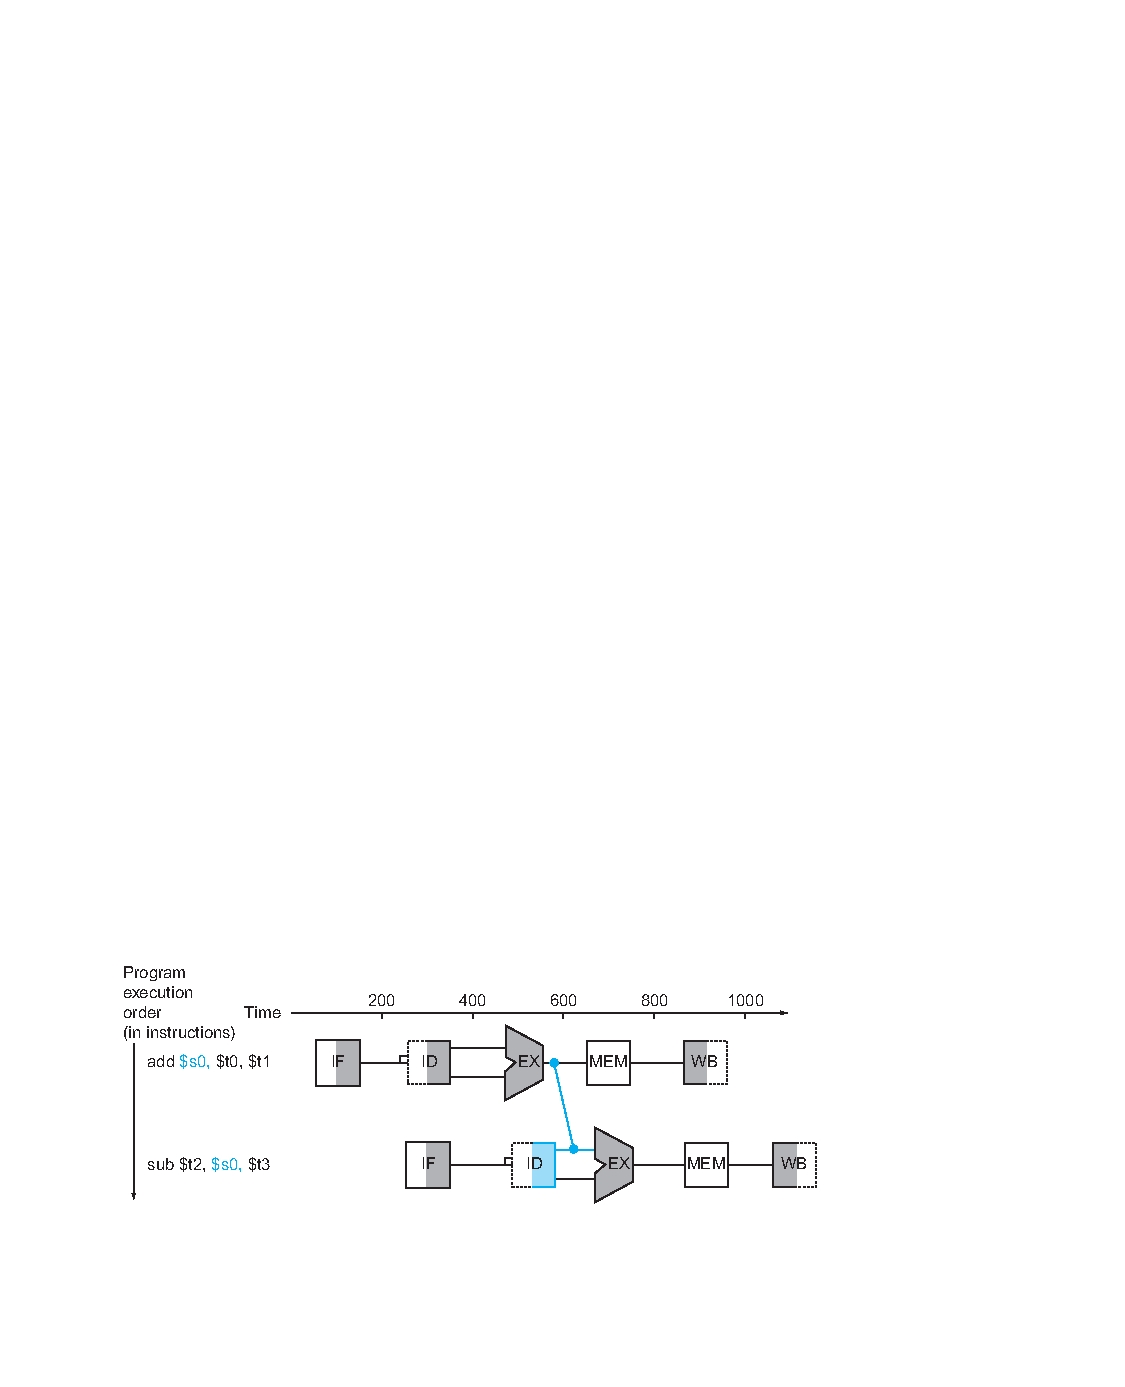
\includegraphics[width=\textwidth]{images/raw_fwd_pl.pdf}
            \label{fig:RAW_fwd}
    \end{my-figure}
\end{figure}

There are multiple scenarios regarding where the data is available and where it is needed. Those are described below.\\

\begin{my-list}{Data hazard scenarios}
    \begin{enumerate}
        \item The first instruction (I1) (I-type or R-type) writes to a register ($R_{dest}$) and the second instruction (I2) attempts to perform an operation using $R_{dest}$ as an operand.\\
        \\This way, the value that is about to be written to $R_{dest}$ is available in EX/MEM pipeline register when I2 is in the Execution stage.
        \item The first instruction (I1) (I-type or R-type) writes to a register ($R_{dest})$, another instruction is issued, and finally, the third instruction (I3) attempts to perform an operation using $R_{dest}$.\\
        \\In this case, the needed value is available in the MEM/WB pipeline register when I3 is in the execution stage.
        \item The first instruction writes to $R_{dest}$ and the second one (I2) is a \textbf{store instruction} that inserts the value of $R_{dest}$ into the memory.\\
        \\In this case, the needed value can be forwarded from the MEM/WB pipeline register to the MEM stage of the store instruction. 
        
        \item The first instruction writes to $R_{dest}$, the second one is a "safe" instruction, and the third one is a store instruction that attempts to store the value at $R_{dest}$ in the Register file.
        
        \item The first instruction is a load and the next one is a store that inserts the previously loaded value at a different address.\\
        \\In this case, the data needed to be stored is available in the MEM/WB stage when it is needed (in MEM stage of the store instruction). However, this situation will be solved using the Hazard Detection unit that is designed specifically for the times the first instruction is a load.
    \end{enumerate}
\end{my-list}

\begin{remark}{Forwarding priority}
     An instruction that uses a register previously written needs to get the value most recently written to that register.\\
     \tcblower
     The mechanisms for detecting these situations and generating the control signals are described in the Design section.\\
\end{remark}

\textbf{The Load Data hazard} (LDH) appears in the situation depicted in \ref{fig:ldh_pl}. The bubble or stall represents that the instruction depending on the load (and all the following ones) are delayed for one clock cycle. The state of the register file and the memory must not change after the stall.

\begin{figure}[h]
\begin{my-figure}{Inserting a stall and forwarding for Load Data Hazards ~\cite{patterson2014computer}}
    \centering
    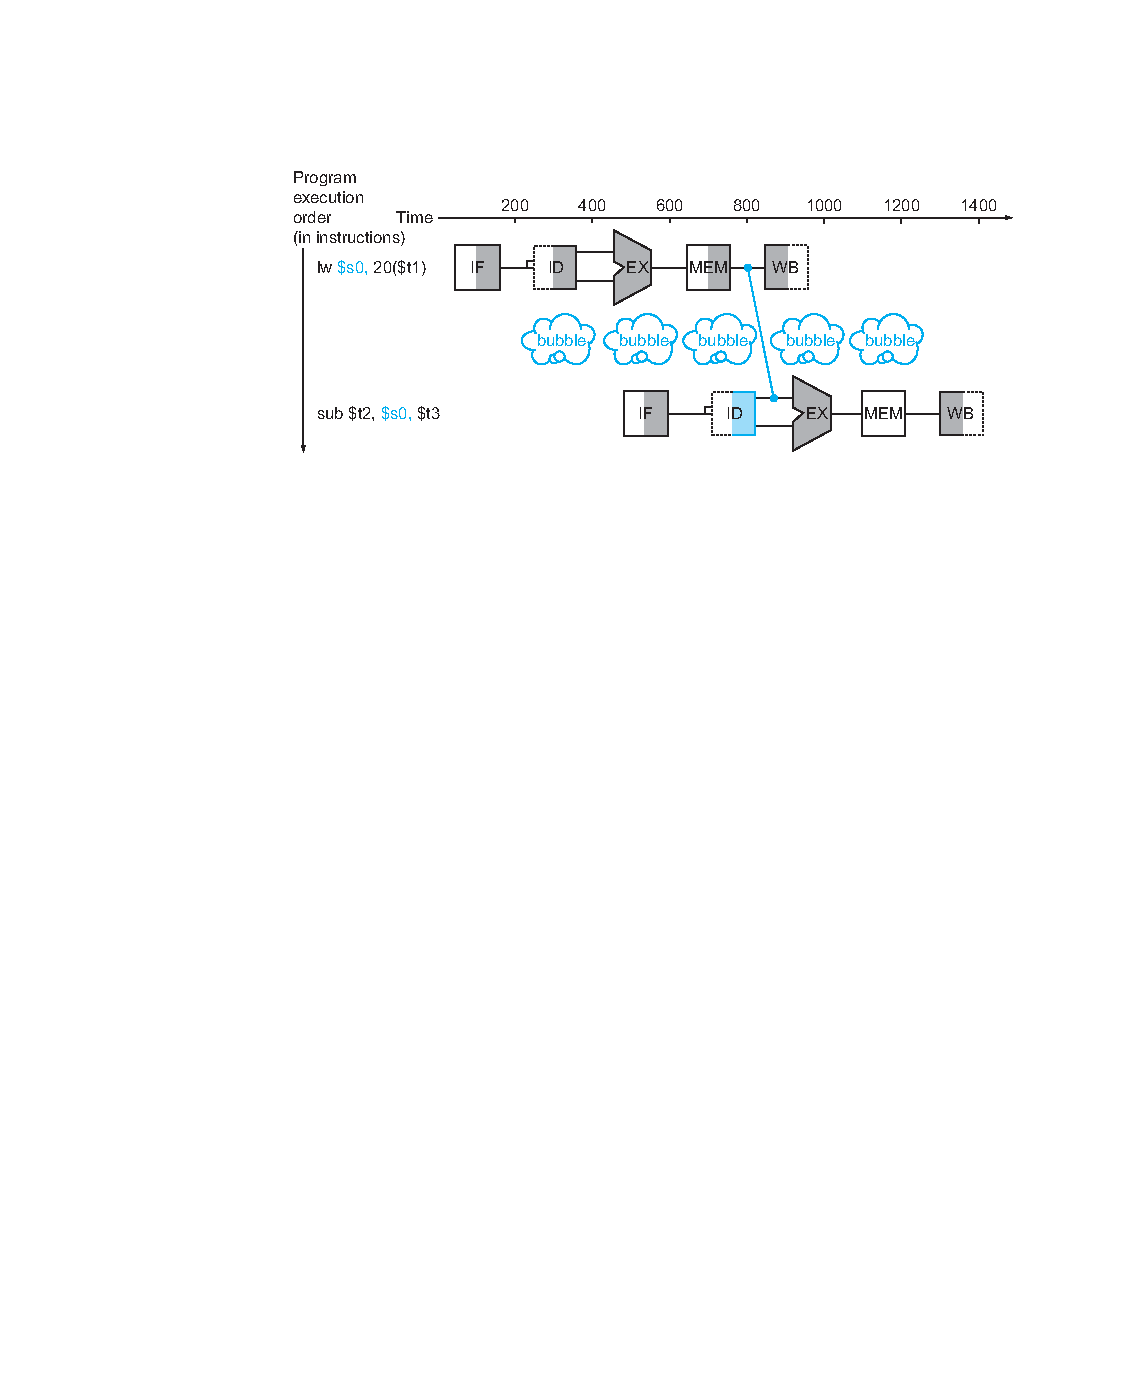
\includegraphics[width=\textwidth]{images/ldh_pl.pdf}
    \label{fig:ldh_pl}
\end{my-figure}
\end{figure}

For the \textbf{control hazards}, we need a hardware mechanism for flushing the instructions after a branch whose correct behavior was not predicted accordingly. To minimize the number of instructions that need to be flushed, the branch detection logic is moved to the Instruction Decode stage. Therefore, only one instruction is started before branch decision is known. So, the flushing mechanism can focus on deleting the data transmitted from the Instruction Fetch Phase to the Instruction Decode Phase through the pipeline register (IF/ID). \\
A dynamic branch prediction method will be implemented to determine the next instruction to be executed.

\subsection{Dynamic Branch Prediction}
Dynamic Branch Prediction uses data obtained during the program execution to predict which instruction to execute next after the current one. 

The chosen approach features a \textbf{branch history table}, a combination between a branch target buffer and a 2-bit predictor table ~\cite{patterson2014computer}. The table accumulates information to predict the next instruction of the program counter. On one hand it keeps a counter that is incremented when a branch is taken and decremented when it is not taken, and on the other hand it keeps the address that was input into the program counter the last time when the branch was taken.

As branch decisions tend to repeat (see loops), this proves a lot better than static prediction (assume branch not taken). Based on the history, the next address inserted in the program counter can either be the branch target, or the next instruction.

\chapter{Design}

The design of the MIPS pipeline on 16 bits is not the object of this project . It is considered to be a fully functional processor (as shown in \ref{fig:pipeline_init}) supporting a fixed set of instruction (see table \ref{table:mips_isa}).

\begin{remark}{Notation}
    \textbf{Note}: the notations of the instructions are:
    \begin{itemize}
        \item \verb|r_ins $dest, $op1, $op2| - for r-type instructions
        \item \verb|i_ins $dest, $op1, imm| - for i-type instructions
        \item \verb|branch $op1, $op2, imm| - for branches
        \item \verb|jmp imm| - for jumps
    \end{itemize}
\end{remark}

\begin{my-table}{Instructions supported by the processor}
    \begin{center}
            \begin{tabular}{|c|c|c|}
                \hline
                \textbf{Instruction} & \textbf{Type} & \textbf{RTL Abstract}\\
                \hline
                \verb|add $rd, $rs, $rt|& R & RF[rd] $\leftarrow$ RF[rs] + RF[rt]\\
                \hline
                \verb|sub $rd, $rs, $rt|& R &RF[rd] $\leftarrow$ RF[rs] - RF[rt]\\
                \hline
                \verb|sll $rd, $rs, $rt|& R & RF[rd] $\leftarrow$ RF[rs] $\ll$ RF[rt]\\
                \hline
                \verb|srl $rd, $rs, $rt|& R & RF[rd] $\leftarrow$ RF[rs] $\gg$ RF[rt]\\
                \hline
                \verb|and $rd, $rs, $rt|& R & RF[rd] $\leftarrow$ RF[rs] $\And$ RF[rt]\\
                \hline
                \verb|or $rd, $rs, $rt|& R & RF[rd] $\leftarrow$ RF[rs] $||$ RF[rt]\\
                \hline
                \verb|xor $rd, $rs, $rt|& R & RF[rd] $\leftarrow$ RF[rs] $\oplus$ RF[rt]\\
                \hline
                \multicolumn{}{}{}\\
                \hline
                \verb|addi $rt, $rs, imm|& I & RF[rd] $\leftarrow$ RF[rs] + $S_{Ext}$(imm)\\
                \hline
                \verb|subi $rt, $rs, imm|& I & RF[rd] $\leftarrow$ RF[rs] - $S_{Ext}$(imm)\\
                \hline
                \verb|lw $rt, $rs, imm|& I & RF[rt] $\leftarrow$ Mem[RF[rs] + $S_{Ext}$(imm)]\\
                \hline
                \verb|sw $rt, $rs, imm|& I & Mem[RF[rs] + $S_{Ext}$(imm)] $\leftarrow$ RF[rt] \\
                \hline
                \verb|beq $rt, $rs, imm|& I & \textbf{if} RF[rs] == RF[rt] \textbf{then}  \\
                & & PC $\leftarrow$ PC + 1 \\
                & & \textbf{else} \\
                & & PC $\leftarrow$ PC + 1 + $S_{Ext}$(imm)\\
                \hline
                \verb|bneq $rt, $rs, imm|& I & \textbf{if} RF[rs] \ne RF[rt] \textbf{then}  \\
                & & PC $\leftarrow$ PC + 1 \\
                & & \textbf{else} \\
                & & PC $\leftarrow$ PC + 1 + $S_{Ext}$(imm)\\
                \hline
                \multicolumn{}{}{}\\
                \hline
                \verb|jmp imm| & J & PC $\leftarrow$ $Ext$(imm) \\
                \hline
        \end{tabular}
        \label{table:mips_isa}
    \end{center}
\end{my-table}

\begin{figure}
    \begin{my-figure}{MIPS Pipeline with no hazard detection and resolution ~\cite{patterson2014computer}}
        \centering
        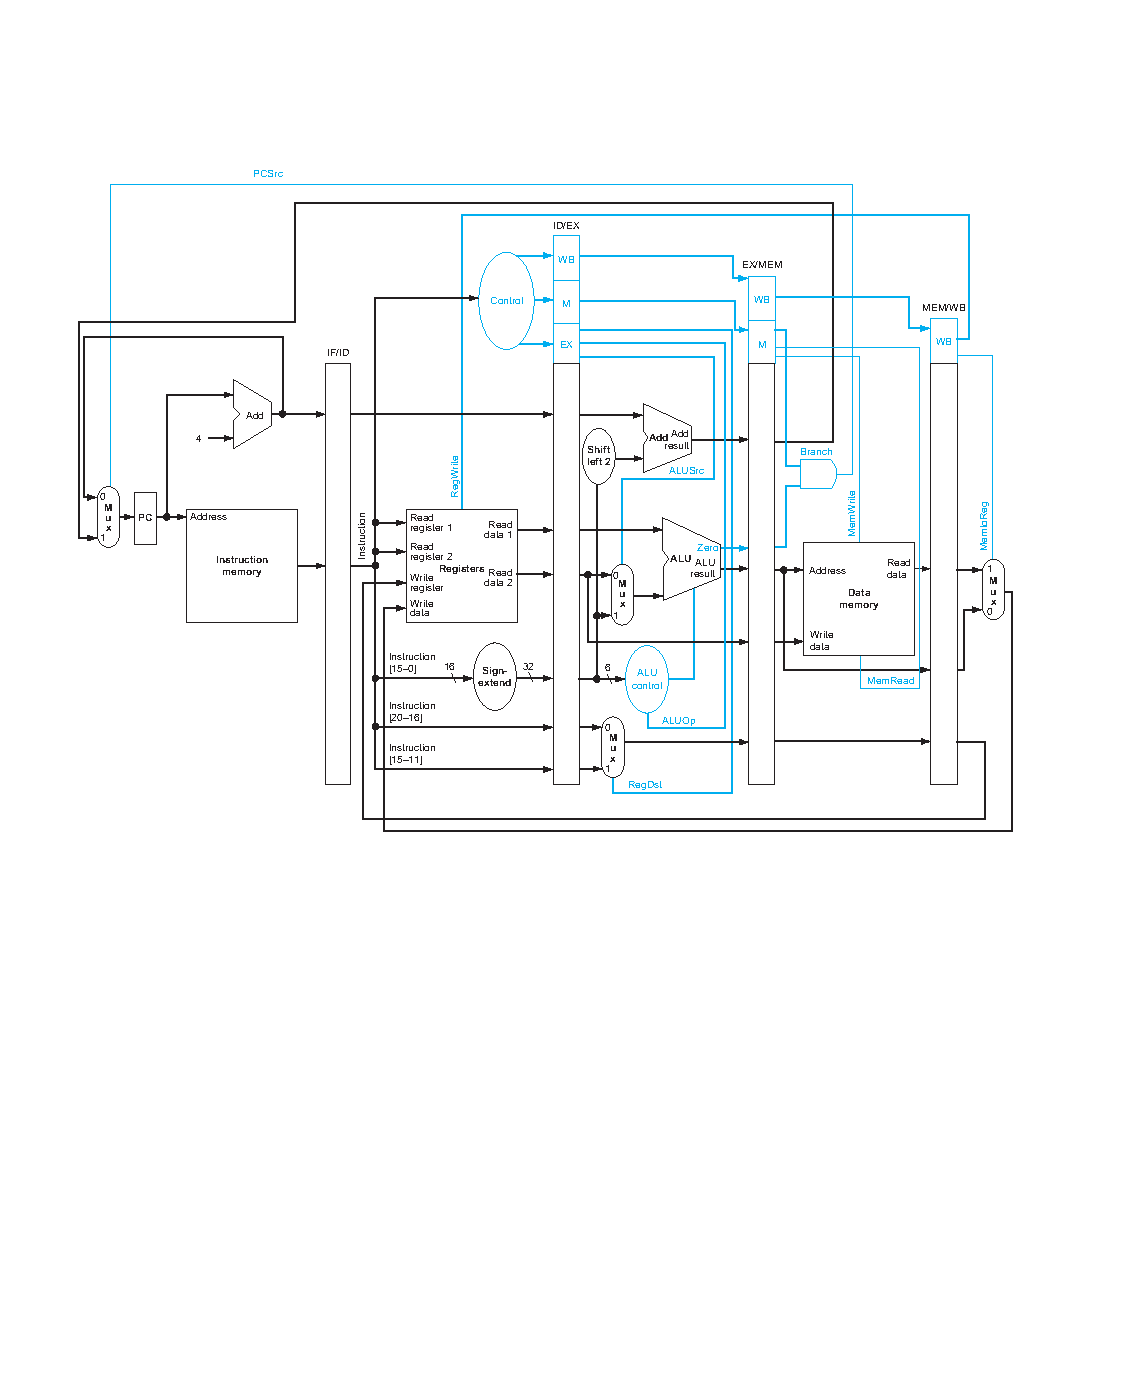
\includegraphics{images/pipeline_mips_initial.pdf}
        \label{fig:pipeline_init}
    \end{my-figure}
\end{figure}

\section{Forwarding Unit Design}
The main goal of this unit is to generate control signals that determine data forwarding, based on some tested conditions. The decision whether to select the forwarded data in the needed context is taken by the forwarding unit.\\
The different cases that were presented in the Project Analysis section are solved as it is covered below.\\
\begin{remark}{Notations for signals}
    \begin{itemize}
        \item Pipeline\_Stage/Next\_Pipeline\_Stage refers to the pipeline registers between the two stages
        \item Register Rs refers to the address of the first operand of the R and I type instructions
        \item Register Rt refers to the address of the second operand of the R-type instruction and the address of the destination of the I-type instruction.
        \item RegWrite signal is the control signal generated by the Control Unit that determines writing in the register file.
    \end{itemize}
\end{remark}
\subsection{Forwarding from the previous instruction}
In this case, the forwarding unit needs to have information regarding the following signals:
\begin{my-list}{EX Forwarding unit inputs}
    \begin{itemize}
        \item ID/EX\_Rs
        \item ID/EX\_Rt
        \item EX/MEM\_RegDest
        \item EX/MEM\_RegWrite
        \item EX/MEM\_ALUOut
    \end{itemize}
\end{my-list}
The forwarded data will be taken from EX/MEM\_ALUOut and sent to the ALU input corresponding to Rs (Input A) or Rd (Input A). Two additional Multiplexers are added to ensure the correctness of the forwarding, and the forwarding unit is placed in the EX stage.\\
The selections of these multiplexers are the output signals of the Forwarding unit.

\begin{my-list}{EX Forwarding unit outputs}
    \begin{itemize}
        \item ForwardA - on two bits so far, if 1 it determines the ALU input A to be the forwarded data, otherwise ordinary data is sent there
        \item ForwardB
    \end{itemize}
\end{my-list}
The conditions for determining data forwarding are described in the following listing.

\begin{my-listing}{Conditions for forwarding from EX/MEM refister}
    \begin{lstlisting}[style=vhdl]
if (EX/MEM_RegWrite == 1) && (ID/EX_Rs == EX/MEM_RegDest) then
    ForwardA = 1;
    
if (EX/MEM_RegWrite == 1) && (ID/EX_Rt == EX/MEM_RegDest) then
    ForwardB = 1;
    \end{lstlisting}
\end{my-listing}

\subsection{Forwarding from the instruction before the previous}
The inputs necessary for the forwarding unit are:
\begin{my-list}{More inputs for the EX forwarding unit}
    \begin{itemize}
        \item MEM/WB\_RegWrite
        \item MEM/WB\_ALUOut
        \item MEM/WB\_RegDest
    \end{itemize}
\end{my-list}
The outputs of the forwarding unit in this sense, are like in the previous case, selection bits of the multiplexers that determine the ALU inputs. Consequently we need to extend the width of the ForwardA and ForwardB signals to 2 bits.
The meaning of the bits assigned to the ForwardA and ForwardB outputs is described in the table below.

\begin{my-table}{The meaning of the bits assigned to ForwardA or ForwardB}
    \begin{center}
    \begin{tabular}{|c|c|c|}
        \hline
        \textbf{Assigned value} & \textbf{Consequence}\\
         \hline
         00 &  ALU input is \textbf{not} represented by forwarded data\\
        \hline
         01 &  ALU input is forwarded from \textbf{EX/MEM} pipeline register\\
        \hline
         10 &  ALU input is forwarded from \textbf{MEM/WB} pipeline register\\
        \hline
         11 &  -\\
        \hline
    \end{tabular}
    \end{center}
    \label{table:1}
\end{my-table}

The conditions for forwarding from MEM/WB stage are presented below.

\begin{my-listing}{Forwarding from MEM/WB register}
    \begin{lstlisting}[style=vhdl]
if (MEM/WB_RegWrite == 1) && (ID/EX_Rs == MEM/WB_RegDest) then
    ForwardA = 10;
    
if (MEM/WB_RegWrite == 1) && (ID/EX_Rt == MEM/WB_RegDest) then
    ForwardB = 10;
    \end{lstlisting}
\end{my-listing}

One \textbf{mention} needs to be made. We might have data dependency between the instruction currently executed and the instruction before the previous one, but there may be another dependency between the current instruction and the one immediately previously executed. Therefore the most recent result (stored in the EX/MEM register) needs to be forwarded. This issue will be solved in the VHDL implementation.

To put it all together, the additional hardware changes so far (in blue) are shown in \ref{fig:fwd_ex}.

\begin{figure}[h]
    \begin{my-figure}{Hardware Modifications for forwarding in the Execution Stage}
        \centering
        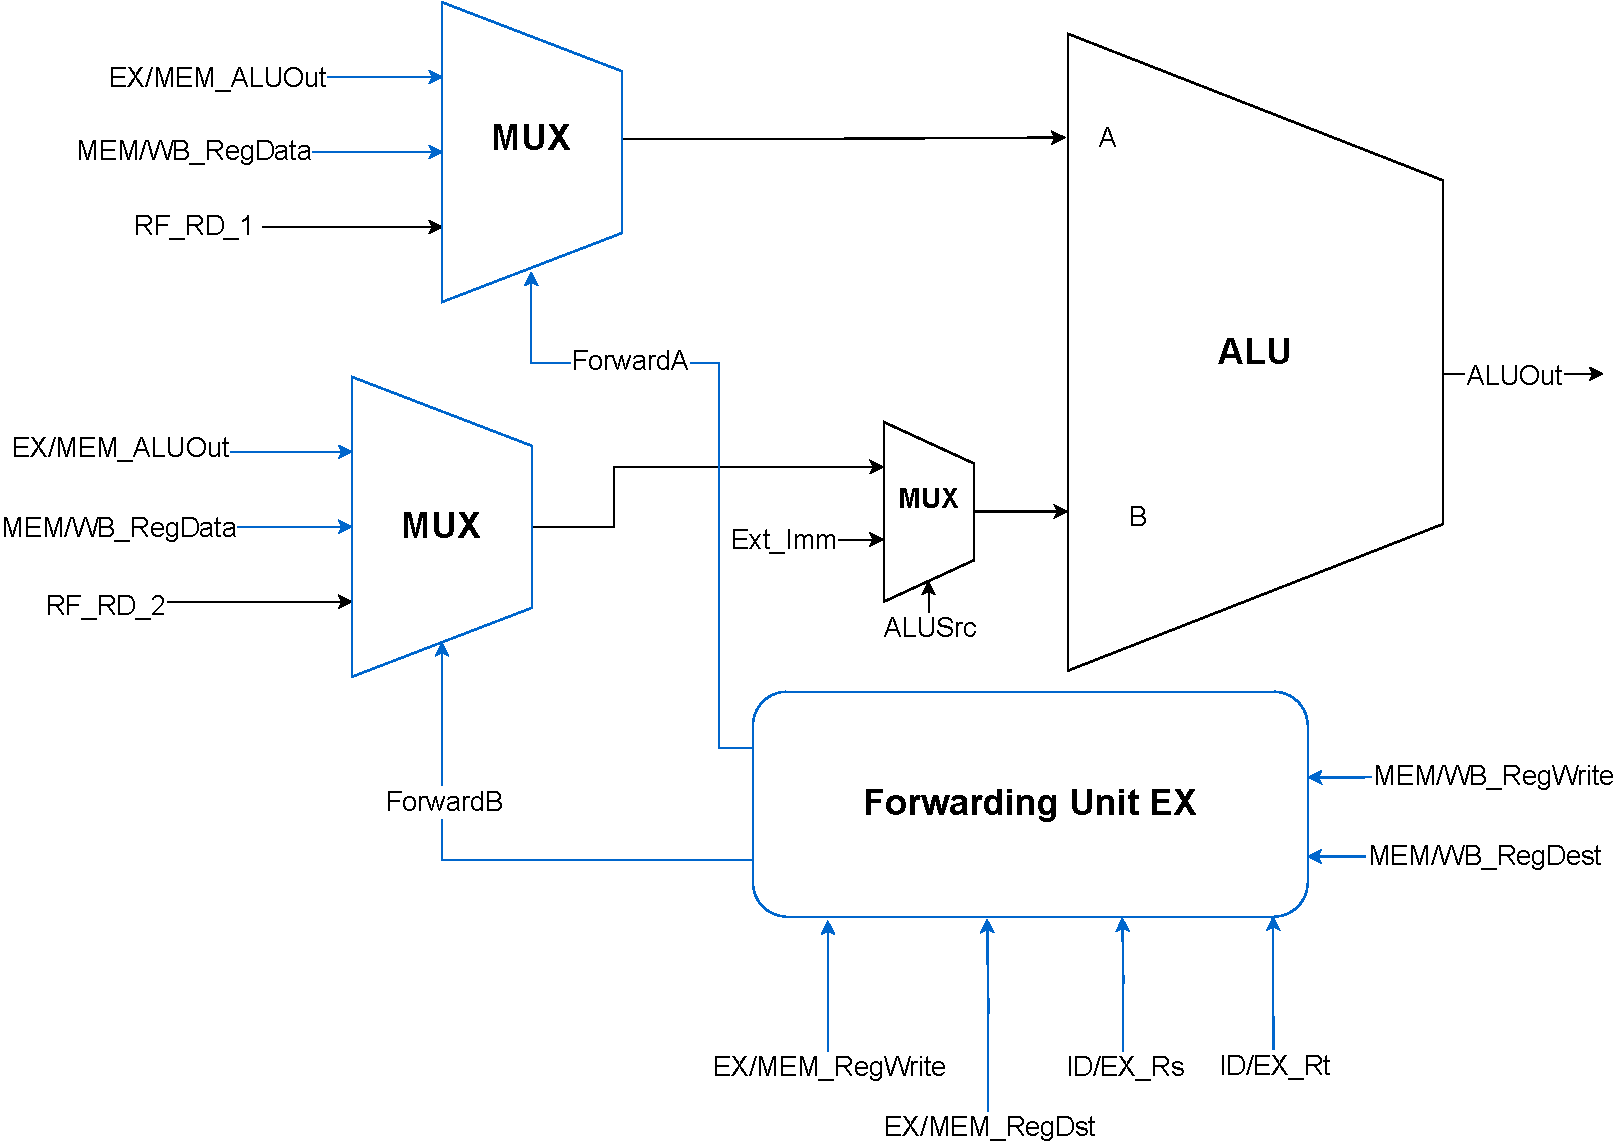
\includegraphics[width=0.7\textwidth]{images/fwd_ex.pdf}
        \label{fig:fwd_ex}
    \end{my-figure}
\end{figure}

\subsection{Forwarding to the MEM stage}
This situation imposes forwarding data to the data entry of the Data Memory, therefore, another forwarding unit (Forwarding Unit MEM) placed in the MEM stage is necessary. 

\subsubsection{Forwarding from the previous instruction}
In the case the data dependency comes from the previous instruction, the inputs of the forwarding unit are:
\begin{my-list}{MEM Forwarding unit inputs}
    \begin{itemize}
        \item EX/MEM\_Rt - that was not previously sent to the MEM stage, but is needed now.
        \item EX/MEM\_MemWrite - that shows that the current instruction is a store.
        \item MEM/WB\_RegWrite
        \item MEM/WB\_RegDst
    \end{itemize}
\end{my-list}

The output is a selection (\textbf{ForwardC}) of a multiplexer that determines to introduce either the forwarded content from the WB stage of the previous instruction, or the usual data that is written to the memory (content of the register file at Rt address).

The new forwarding unit keeps a similar structure to the one from the execution stage and the condition for generating the forwarding signal is:

\begin{my-listing}{Forwarding to MEM from MEM/WB register}
    \begin{lstlisting}[style=vhdl]
if (MEM/WB_RegWrite == 1) && (EX/MEM_Rt == MEM/WB_RegDest) && (EX/MEM_MemWrite) then
    ForwardC = 1;
    \end{lstlisting}
\end{my-listing}

\subsubsection{Forwarding from the instruction before the previous one}
This is a special case as the information regarding the address of the register file where the instruction before the previous one wrote and the control signal that enabled the writing have already passed through the whole pipeline and are no longer available as depicted in the following table.

The solution is to buffer this information for one more clock cycle to be able to use the forwarding unit in the memory stage. This buffer register is called \textbf{WB\_BUF}. So the signals available to the forwarding unit are:

\begin{my-list}{Additional inputs for the forwarding unit}
    \begin{itemize}
        \item WB\_BUF\_RegDst
        \item WB\_BUF\_RegWrite
    \end{itemize}
\end{my-list}

In addition, the WB\_BUF\_RegData (data that was written to the Register File at the WB\_BUF\_RegDst address) needs to be buffered so that it can be forwarded to the data input of the Data Memory.

The multiplexer placed at the entrance of the data memory now has 3 inputs, so ForwardC signal is expanded to 2 bits having the meanings described in Table 4.3.

\begin{my-table}{The meaning of the bits assigned to ForwardC}
    \begin{center}
    \begin{tabular}{| m{6em} | m{10cm} |}
        \hline
        \textbf{Assigned value} & \textbf{Consequence}\\
         \hline
         00 &  Data Memory data input is \textbf{not} represented by forwarded data\\
        \hline
         01 &  Data Memory data input is forwarded from \textbf{MEM/WB} pipeline register\\
        \hline
         10 &  Data Memory data input is forwarded the from \textbf{WB\_BUF} register\\
        \hline
         11 &  -\\
        \hline
    \end{tabular}
    \end{center}
    \label{table:1}
\end{my-table}

\begin{my-listing}{Forwarding to MEM from WB\_BUF register}
    \begin{lstlisting}[style=vhdl]
if (WB_BUF_RegWrite == 1) && (EX/MEM_Rt == WB_BUF_RegDest) && (EX/MEM_MemWrite) then
    ForwardC = 10;
    \end{lstlisting}
\end{my-listing}

The same observation regarding the importance of forwarding the most recent modification of RegDst holds in this case. Once again, this will be solved in the VHDL implementation. The hardware modifications and additions (in blue) are shown in \ref{fig:fwd_mem}

\begin{figure}
\begin{my-figure}{Hardware Modifications for forwarding in the Memory Stage}
    \centering
    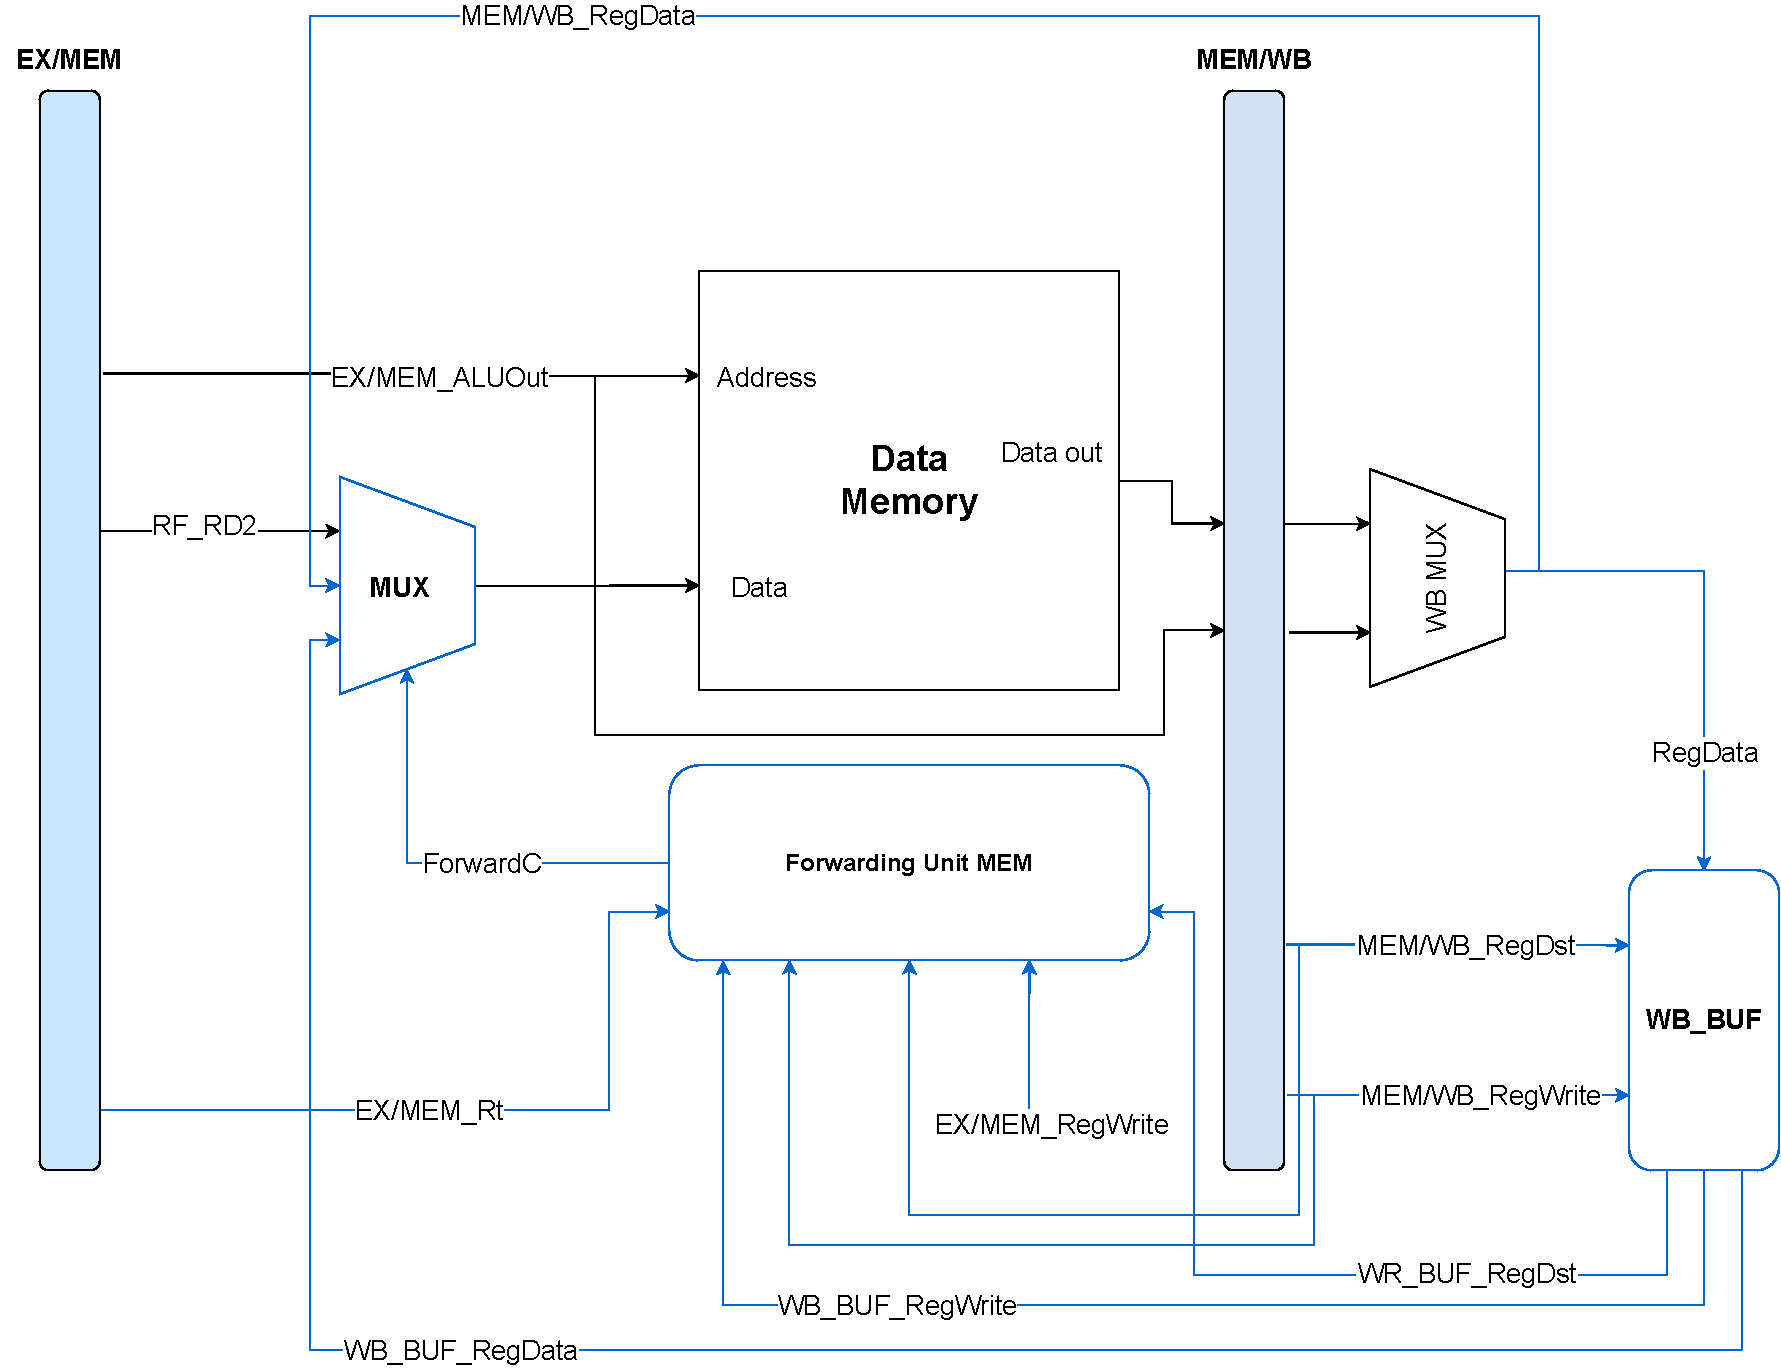
\includegraphics[width=0.8\textwidth]{images/fwd_mem.pdf}
    \label{fig:fwd_mem}
\end{my-figure}
\end{figure}

\section{Hazard detection Unit Design}
This component detects with the special case of \textbf{load data hazards} described in the Project Analysis section. It needs to detect the dependency between the currently executing instruction (that is already in the ID stage) and the previous one that in this case needs to be a load for the bubble to be inserted.

The information necessary for the hazard to be detected is:
\begin{my-list}{HDU Inputs}
    \begin{itemize}
        \item ID\_Rt
        \item ID\_Rs
        \item ID/EX\_Rt - the register file location where the loaded data from memory will be stored.
        \item ID/EX\_MemRead - HIGH only when the instruction is a load.
    \end{itemize}
\end{my-list}

The condition for a load to be detected is presented in the listing below.

\begin{my-listing}{Detecting a load data hazard}
\begin{lstlisting}[style=vhdl]
if (ID/EX_MemRead == 1) && 
    ( (ID/EX_Rt == ID_Rt) || (ID/EX_Rt == ID_Rs) ) then
    insert bubble;
    \end{lstlisting}
\end{my-listing}

The mechanism of stalling the pipeline is achieved by making sure that the register file and the data memory is not modified. Therefore, the control signals generated for instruction currently in ID stage will be pulled to 0 by the Hazard Detection Unit (with the aid of a multiplexer). 

Moreover, the state of the instruction in the ID stage needs to be frozen, so the IF/ID pipeline register needs to maintain its state. This is achieved by adding an enable signal that would prevent the instruction in IF stage to overwrite the IF/ID register. 

Finally, the instruction currently in IF stage needs to be issued again after a clock cycle so the program counter will be also stopped by using an enable signal.

With this in mind, the outputs of the hazard detection unit and their meaning are listed in \ref{table:hdu_out}.

\begin{my-table}{The outputs of the Hazard Detection Unit and their meaning}
    \centering
    \begin{tabular}{|c|c|c|}
        \hline
        \textbf{Output} & \textbf{on HIGH} & \textbf{on LOW}\\
         \hline
         PC\_Enable & No hazard, normal counting & LDH detected, freeze the counting\\
        \hline
         Ctrl\_SEL & No hazard, send control signals & LDH detected, send zeros \\
        \hline
         IF/ID\_Enable & No hazard, send IF data & LDH detected, preserve reg. state  \\
        \hline
    \end{tabular}
    \label{table:hdu_out}
\end{my-table}

As mentioned in the Project analysis, the load data hazard resolution solves the situation where a store attempts to insert to memory what has been previously loaded from another memory location. In this situation, a stall is inserted after the load.  Afterwards, the situation is solved by forwarding unit (the case where data is forwarded from WB\_BUF to MEM stage).

The hardware modifications are shown in \ref{fig:hdu}.

\begin{figure}
    \begin{my-figure}{The hazard detection unit and the added signals ~\cite{patterson2014computer}.}
        \centering
        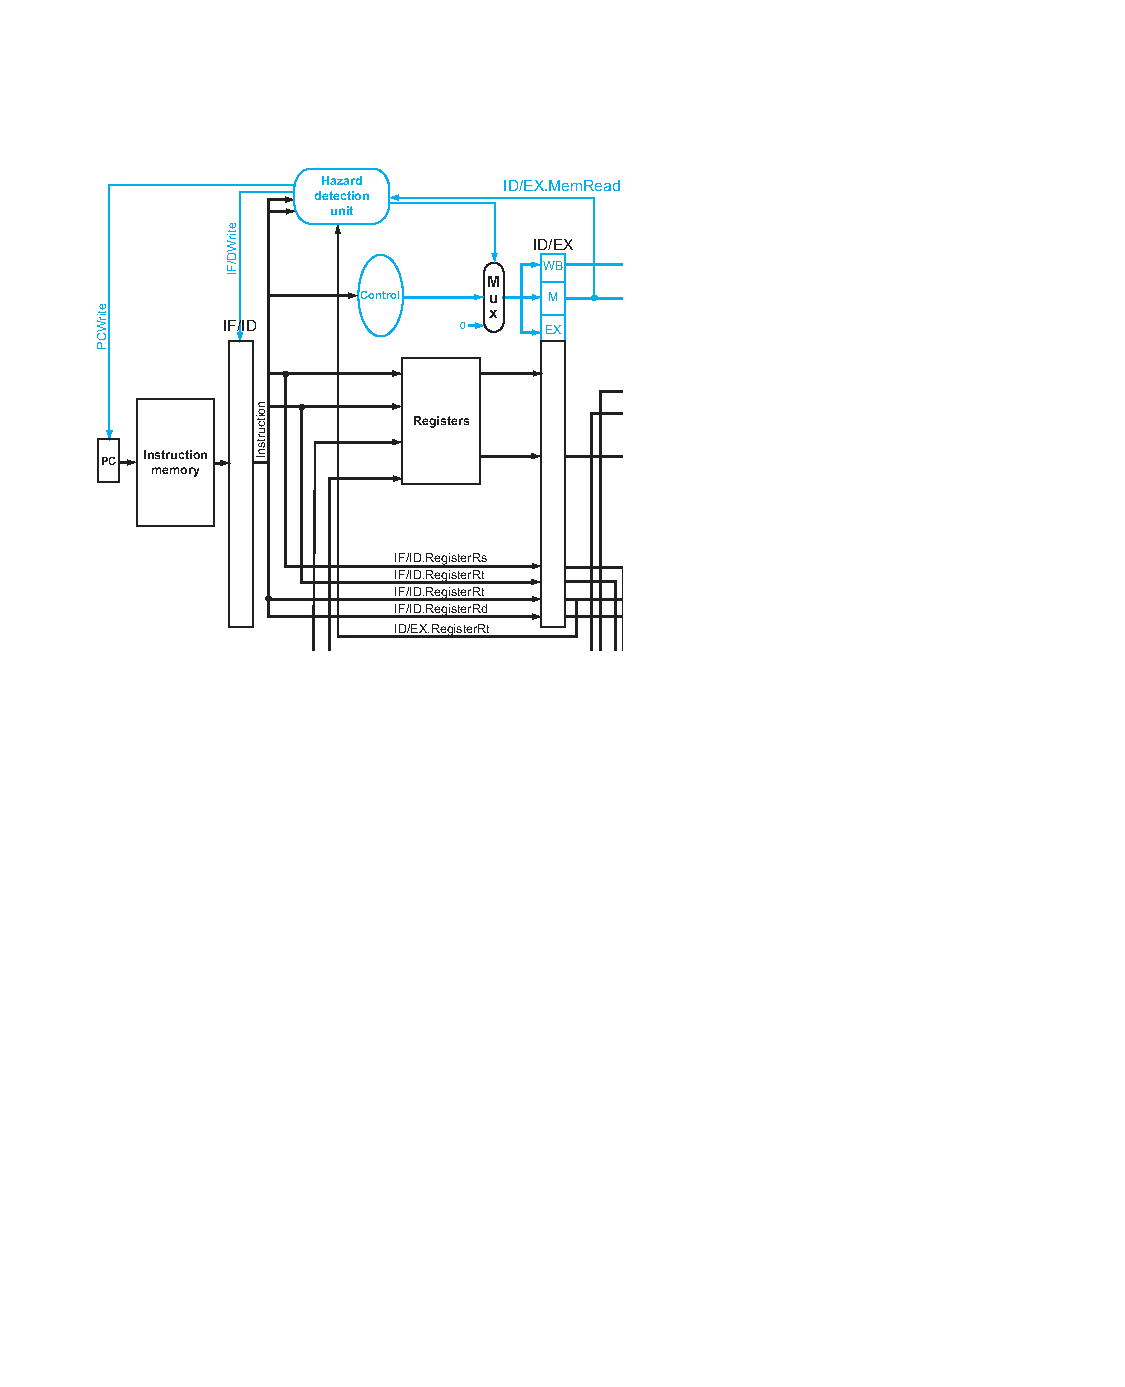
\includegraphics[width=0.7\textwidth]{images/hdu.pdf}
        \label{fig:hdu}
    \end{my-figure}
\end{figure}

\section{Branch Prediction Unit Design}
This unit involves three design steps: moving the branch detection logic and address computation to the ID stage to minimize the number of instructions executed before knowing the branch decision is known, flushing the instructions that were not supposed to be executed, and predicting the branch dynamically according to a history table.
\subsection{Minimize the number of instruction executed after the branch}
In \ref{fig:pipeline_init} there can bee seen that the branch control signal is generated late in the MEM stage. Therefore, supposing a branch is taken and it was predicted not to be taken, three other instructions enter the pipeline. As they must not be performed they need to be flushed and 3 clock cycles that could have generated results are lost.

Minimizing the number of such instruction proves, then, useful. In this design, that will be achieved by generating the branch signal in the ID stage and performing the comparison between the data read from the register file (as in this architecture we will only support branch on equal).

The condition for generating the branch signal (branch\_sel) is:
\begin{my-listing}{Condition for generating the branch taken signal}
\begin{lstlisting}[style=vhdl]
if (Branch == 1) && (RF_RD1 == RF_RD2) then
    branch_sel = 1;
\end{lstlisting}
\end{my-listing}

As it can be seen in the previous section, the values read from the register file might not be correct due to data dependency, therefore moving the branch in the ID stage implies adding forwarding logic to this stage as well. Moreover, data dependencies between the branch (ID) and the previous instruction (EX) can not be resolved without a stall, so the Hazard detection unit needs to be extended to detect this case.

\subsubsection{Extending the Hazard Detection Unit} 
First of all, the inputs needed to be added to detect dependencies to an instruction previously executed are:

\begin{my-list}{Additional inputs for HDU}
    \begin{itemize}
        \item ID\_Branch - the signal generated by the control unit in ID.
        \item ID/EX\_RegWrite
        \item ID/EX\_RegDst
        \item ID\_Rs - address of the first register to be read from RF.
        \item ID\_Rt - address of the second register to be read from RF.
    \end{itemize}
\end{my-list}

So, another stall condition is added to the HDU.

\begin{my-listing}{Stalling because of a branch dependent on another instruction}
    \begin{lstlisting}[style=vhdl]
if (ID_Branch == 1) && (ID/EX_RegWrite == 1) &&
    ((ID/EX_RegDst == ID_Rs) || (ID/EX_RegDst == ID_Rt)) then stall
    \end{lstlisting}
\end{my-listing}

One more  case is when the previous instruction is a load and the destination of the load is a register used in branch detection. 

In this case, the load data hazard described in 4.3 is detected and a first stall is inserted. However, the forwarding still can not be performed, one more stall needs to be inserted.

The condition for inserting the other stall is:

\begin{my-listing}{Stalling because of a branch dependent on a load instruction}
\begin{lstlisting}[style=vhdl]
if (ID_Branch == 1) && (EX/MEM_MemRead == 1) && (EX/MEM_RegWrite) &&
    ((EX/MEM_RegDst == ID_Rs) || (EX/MEM_RegDst == ID_Rt)) then stall
\end{lstlisting}
\end{my-listing}

The addditional inputs of the HDU are:
\begin{my-list}{More HDU inputs}
\begin{itemize}
    \item EX/MEM\_RegDst
    \item EX/MEM\_MemRead
\end{itemize}
\end{my-list}

After the two stalls, the second forwarding condition described in the next section will be met and loaded data will be forwarded.

Note: the first condition check must be the load data hazard, and then the branch-related ones.

\subsubsection{Forwarding Unit ID}
One condition when forwarding to the ID stage is necessary is when the data dependency is between the branch and the previous instruction after stalling.
The inputs of the forwarding unit are:

\begin{my-list}{Inputs of the forwarding unit}
    \begin{itemize}
        \item EX/MEM\_RegWrite
        \item EX/MEM\_RegDst
        \item ID\_Branch
        \item ID\_Rs
        \item ID\_Rt
    \end{itemize}
\end{my-list}

The outputs are selections of the multiplexers that determine what are the inputs of the comparator detecting the branch on equal signal.

\begin{my-listing}{Condition for forwarding to ID stage}
    \begin{lstlisting}[style=vhdl]
if (ID_Branch == 1) && (EX/MEM_RegWrite == 1) &&
    (EX/MEM_RegDst == ID_Rs) then
    ForwardBranchA = 1;

if (ID_Branch == 1) && (EX/MEM_RegWrite == 1) &&
    (EX/MEM_RegDst == ID_Rs) then
    ForwardBranchB = 1;
    \end{lstlisting}
\end{my-listing}

\subsection{Mechanism for flushing}
Now that branch decision is known in ID stage it means that another instruction was issued in the IF stage. This instruction was chosen based on the \textbf{dynamic branch prediction mechanism} (described next). If this mechanism fails the instruction needs to have no effect on the CPU resources.

For this case the Flush signal will be generated and it will empty up the IF/ID register.

All of the hardware modification necessary for moving the branch decision to the ID stage and flushing are shown in \ref{fig:br_fwd_hdu}. For readability, the components and signals that don't influence the branch instruction processing have been omitted.

\begin{figure}[]
\begin{my-figure}{Modifications to the ID stage after moving the branch decision here}
        \centering
        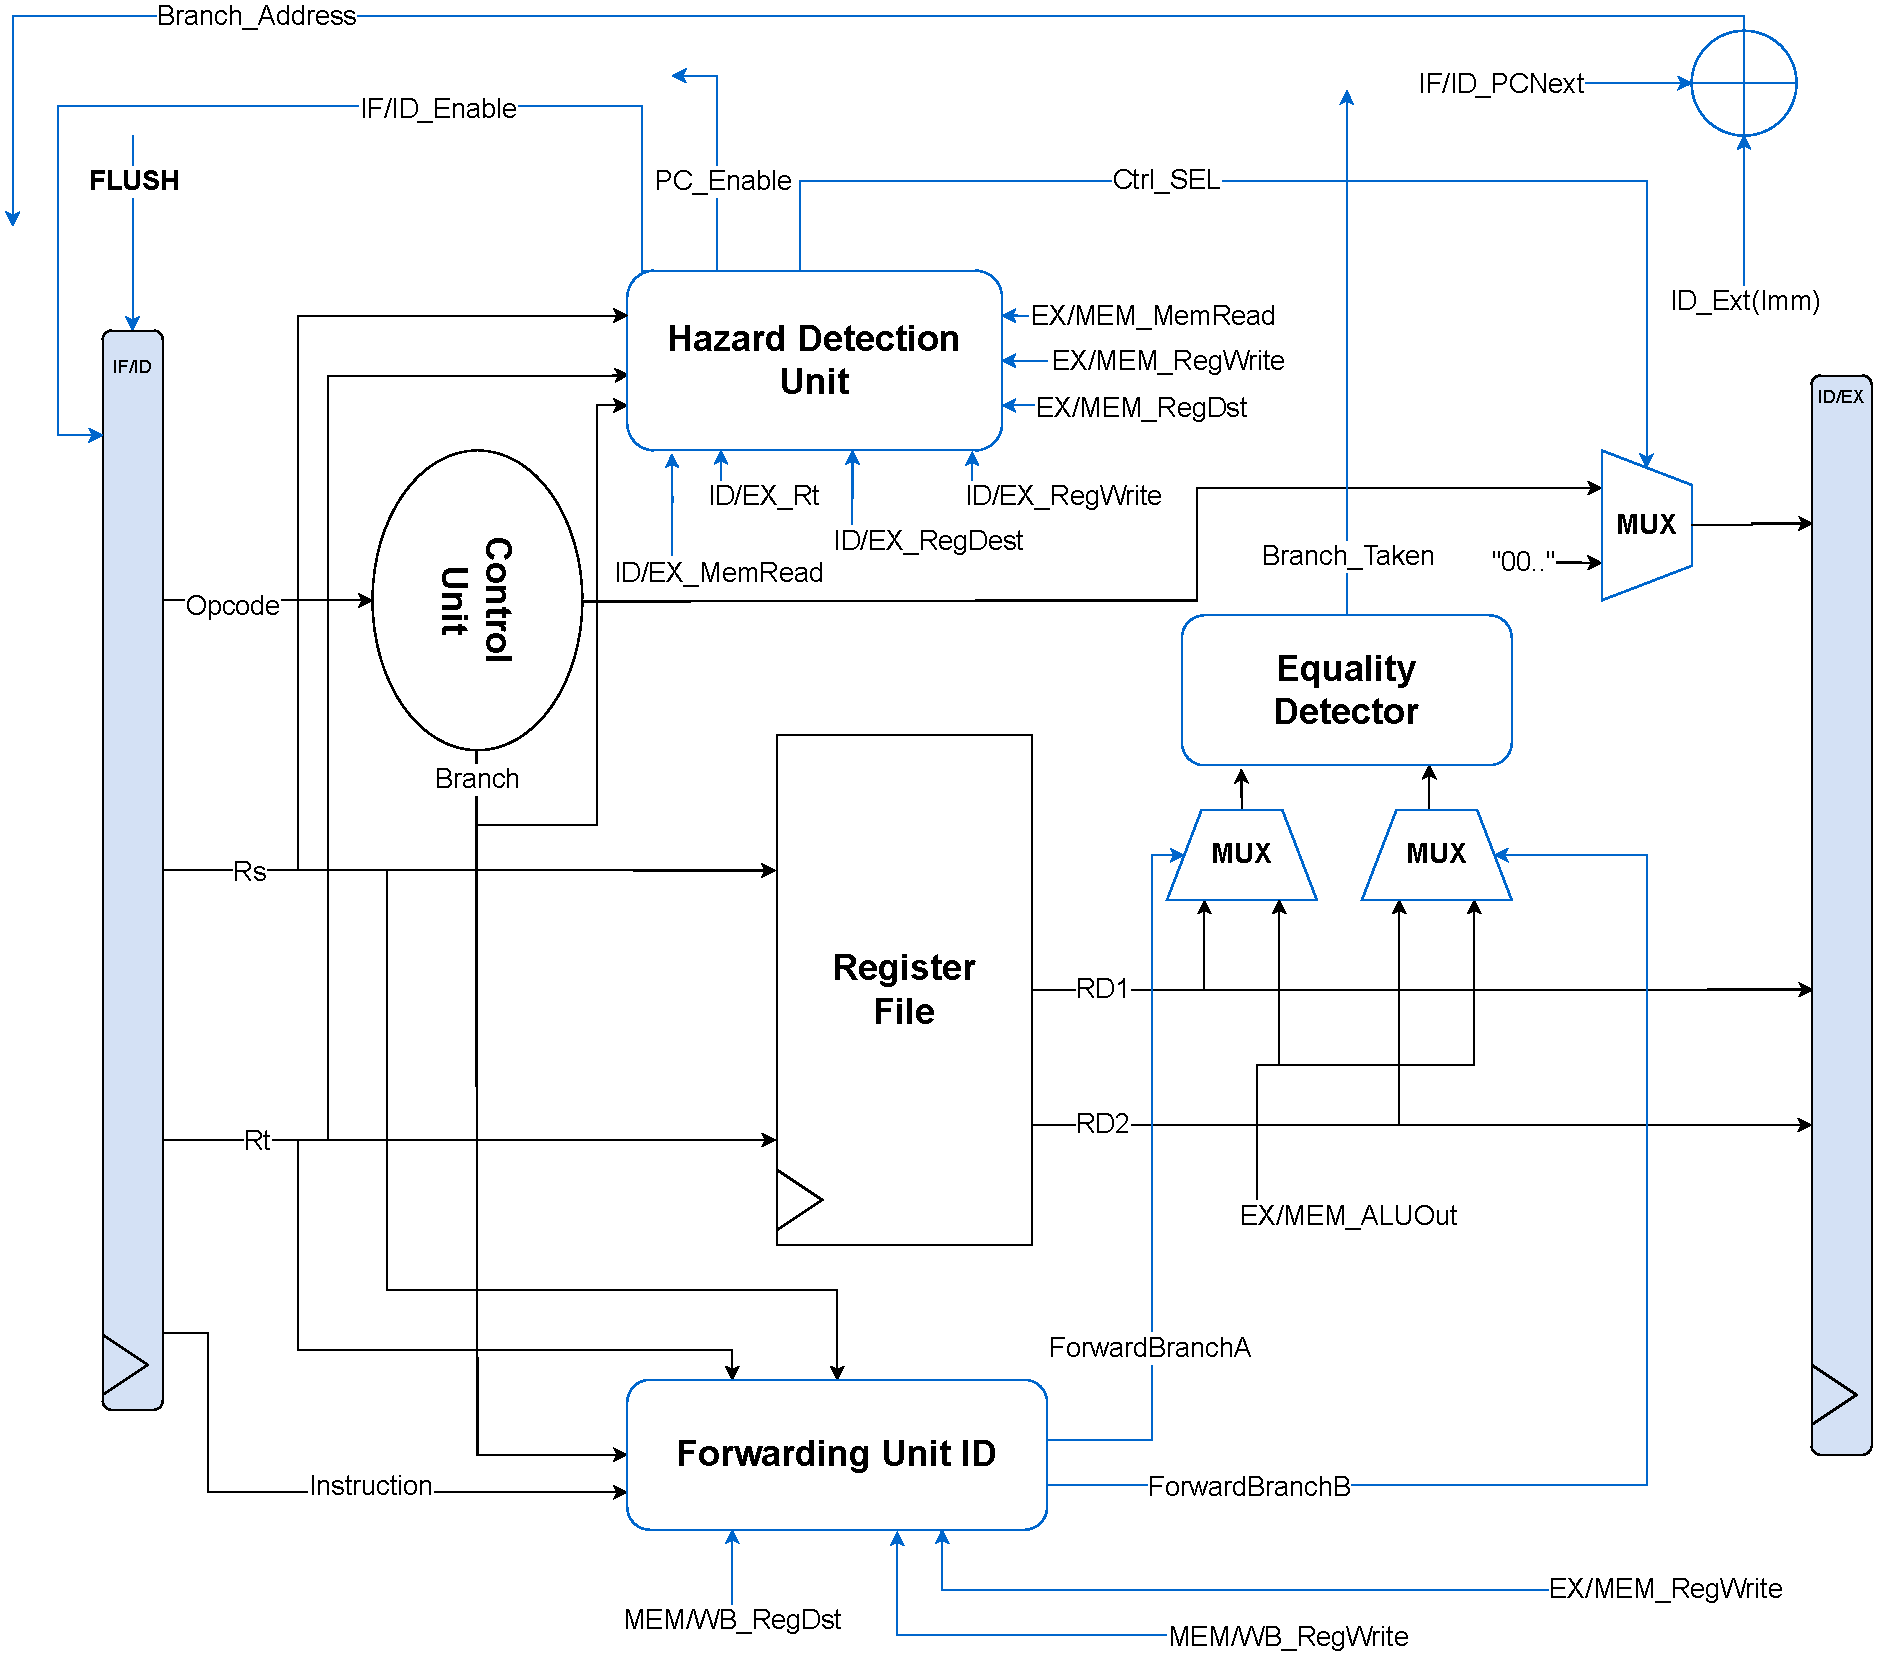
\includegraphics[width=\textwidth]{images/ID_br_fwd_hdu.pdf}
        \label{fig:br_fwd_hdu}
\end{my-figure}
\end{figure}

\subsection{Dynamic branch prediction}
Designing the circuitry that accomplishes dynamic branch prediction involves two stages: read from BHT (Branch history table) and predict (happening in the IF stage), and check prediction and update BHT (that happens in the ID stage after the branch is checked and the branch address is computed).

The structure of the table, shown in \ref{fig:br_pred} as well is similar to the one of a Branch Target Buffer. It is a memory addressed by the lower 4 bits of the program counter address. In a memory entry there is a 2-bit predictor and the target address.

\subsubsection{Read BHT and Predict}
In this step, the next PC address is chosen using the branch history table.

The predictor follows the logic shown in \ref{fig:predictor_fsm}, therefore the MSB detects whether the target address should be input into the PC or not.

\begin{figure}
\begin{my-figure}{Two-bit predictor ~\cite{patterson2014computer}}
    \centering
    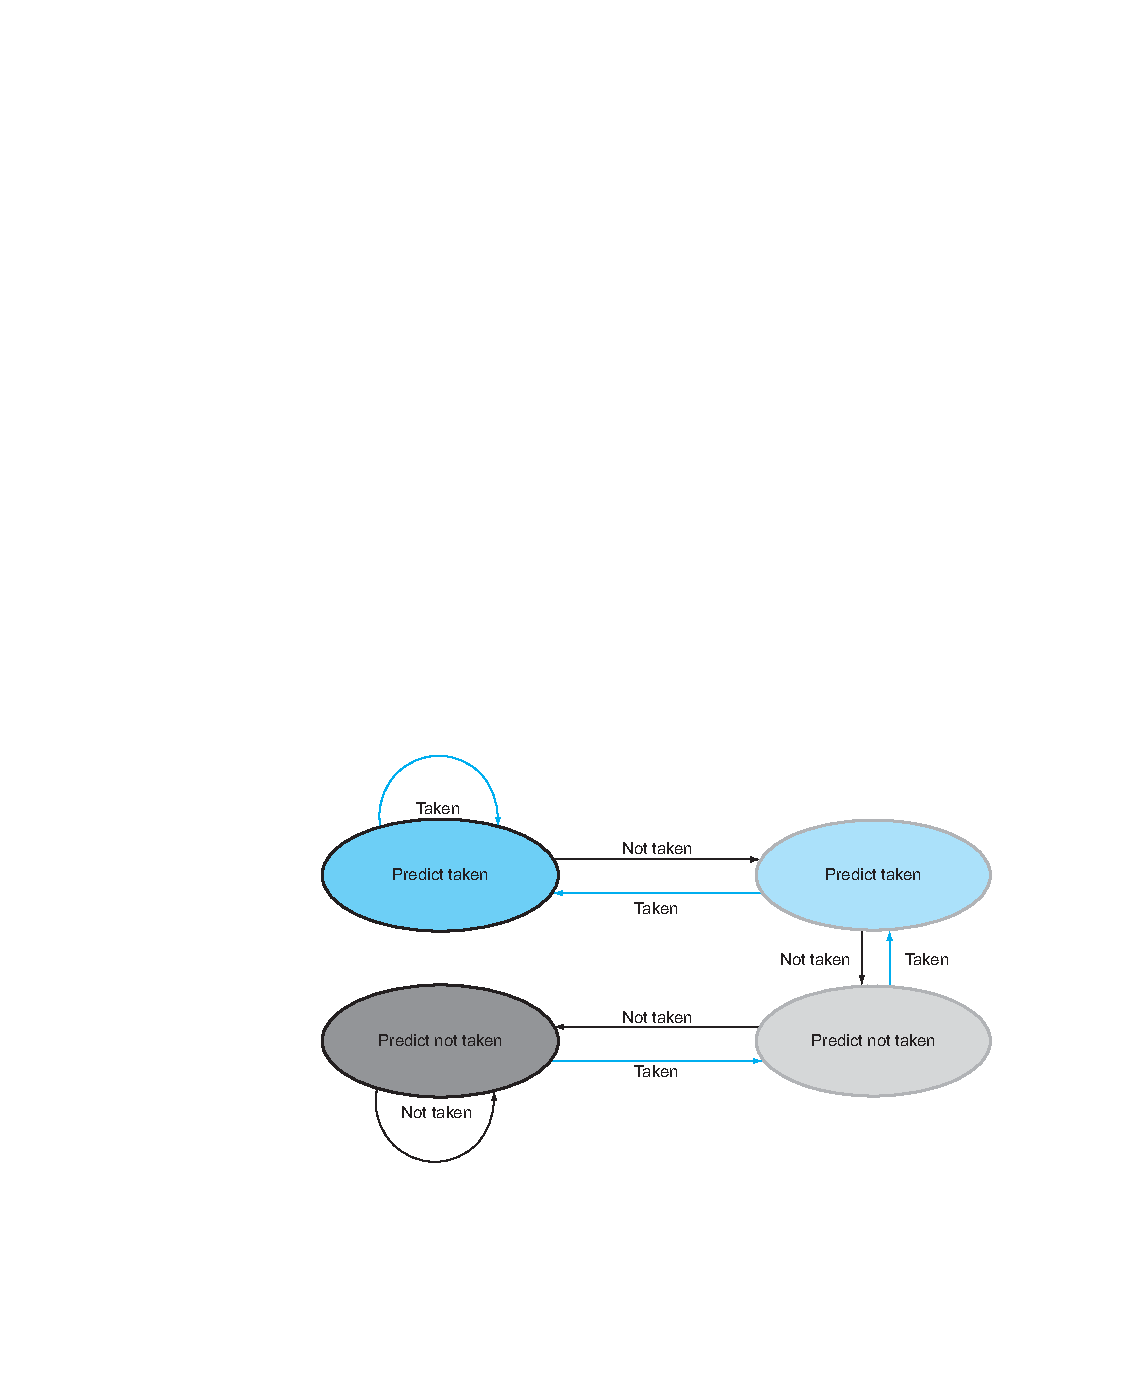
\includegraphics[width=0.7\textwidth]{images/2-bit_pred.pdf}
    \label{fig:predictor_fsm}
\end{my-figure}
\end{figure}
If a branch is predicted, the target address at the same memory address as the predictor is sent to the memory, otherwise the next PC address is \verb|PC + 1| (usual behavior for non-branch instructions).

For the next step (ID) we will send the PC bits that were used to index the BHT to the IF/ID pipeline register, alongside the prediction.

\subsubsection{Check prediction and update BHT}
This stage is reached one clock cycle after the prediction has been made. Now, using the logic added in \ref{fig:br_fwd_hdu} the prediction can be checked.

Checking the prediction is the yields the bit that determines the flush of the IF/ID register. If the Flush condition is determined the next fetched instruction is at the target address computed in the ID.

Now that when the branch outcome is known, the BHT needs to be enriched with this information.
\begin{enumerate}
    \item if the branch was taken the BHT predictor at the address received through the IF/ID register is \textbf{incremented} and the computed branch target address is \textbf{updated to the one newly computed}.
    \item if the branch was \textbf{not} taken, the BHT predictor at the address received through the IF/ID register is \textbf{decremented} (if 0 is reached, it doesn't go below) and the target address is \textbf{not} overwritten.
\end{enumerate}

The design of the dynamic branch prediction (excluding the MIPS components that do not concern this stage) is depicted in \ref{fig:br_pred}

\begin{figure}
    \begin{my-figure}{Hardware additions for the dynamic branch prediction}
        \centering
        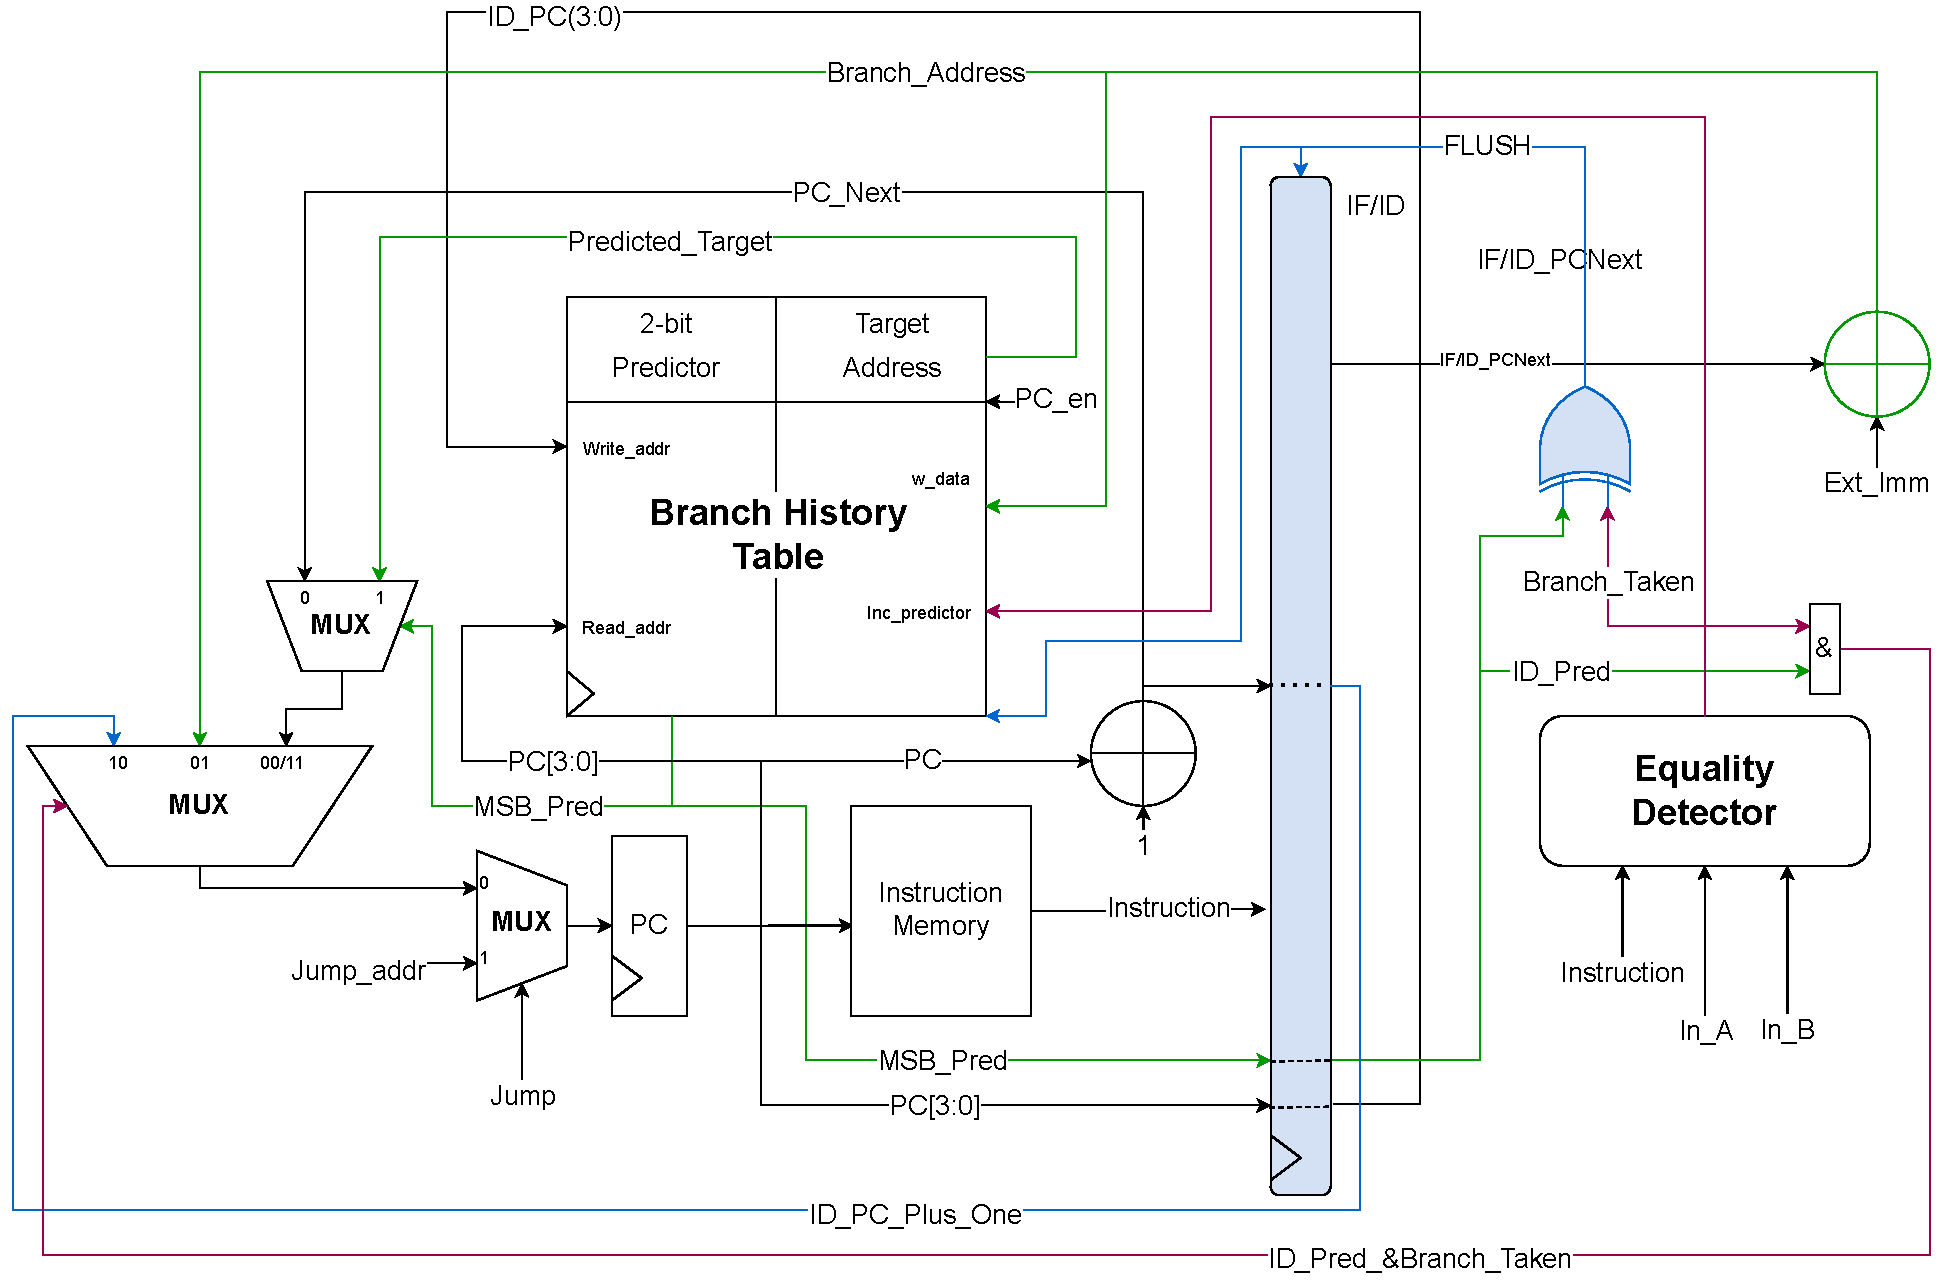
\includegraphics[width=\textwidth]{images/br_pred.pdf}
        \label{fig:br_pred}
    \end{my-figure}
\end{figure}

\chapter{Implementation}
The implementation stage of the Hazard Detection and Avoidance unit starts with adjusting and testing the MIPS pipeline implementation to make sure that it works as expected. Then, the individual components (forwarding units, hazard detection unit) are designed through simple processes that generally check conditions and assign selections for multiplexers.

\section{Changes to the MIPS pipeline implementation}
The MIPS source code written in \textbf{VHDL} is divided into 5 main modules, each one corresponding to a pipeline stage. In addition, the top-level module creates instances of these other modules alongside pipeline registers. \\
However, a few changes need to be made before adding the hazard-handling logic.

\subsection{Reading after writing in the register file}
This modification allows data to be available when, for instance, instruction I1 in ID stage depends on instruction I2 in WB stage. The dependency is detected on the falling edge and data is assigned to the outputs right from the write\_data signal.

\begin{my-listing}{Read after Write in reg\_file.vhd}
    \begin{lstlisting}[style=vhdl]
synchronized: process(clk100MHz)
begin 
   if rising_edge(clk100MHz) then -- writing
       if reg_write = '1' then    
           curr_content(to_integer(unsigned(write_address))) <= write_data; --synchronous write
       end if;
   end if;
   
   if falling_edge(clk100MHz) then -- reading
       read_data1 <= curr_content(to_integer(unsigned(read_address1)));
       read_data2 <= curr_content(to_integer(unsigned(read_address2)));
       
       if read_address1 = write_address and reg_write = '1' then
           read_data1 <= write_data;
       end if;
       
       if read_address2 = write_address and reg_write = '1' then
           read_data2 <= write_data;
       end if;      
   end if;    
end process;
    \end{lstlisting}
\end{my-listing}

\subsection{Adding WB\_BUF register}
For the case shown in \ref{fig:fwd_mem}} we find the need to buffer some of the output signals of the WB stage in an additional pipeline register.

\begin{my-listing}{Adding a new pipeline register in mips16\_top\_sim.vhd}
    \begin{lstlisting}[style=vhdl]
WB_unit: WB_w_data <= 
    MEM_WB(31 downto 16) when MEM_WB(36) = '1'
    else MEM_WB(15 downto 0);
    
pl_WB_BUF: process(reset, clk) is
begin
    if reset = '1' then
        WB_BUF(19 downto 0) <= (others => '0');
    elsif rising_edge(clk) then
        WB_BUF(19) <= MEM_WB(35);
        WB_BUF(18 downto 16) <= MEM_WB(34 downto 32);
        WB_BUF(15 downto 0) <= WB_w_data;
    end if;
end process;
    
    \end{lstlisting}
\end{my-listing}

\subsection{Jump Handling in IF}
The jump address and signal computation is moved to the IF stage to avoid introducing an extra instruction in the pipeline (and eventually flushing it).

\begin{my-listing}{Jump handling in IF\_unit.vhd}
    \begin{lstlisting}[style=vhdl]
jump_detection: jump_if <= '1' when (tmp_instruction(15 downto 13) = "111") else '0'; -- jump
zero_ext: jump_addr_if <= "000" & tmp_instruction(12 downto 0);

mux2: nxt_pc <= jump_addr_if when (jump_if = '1') else mux1_out;    
    \end{lstlisting}
\end{my-listing}

\section{Forwarding Unit}
There are three forwarding units (placed in the IF\_unit, ID\_unit, and MEM\_unit) and implemented according to the design chapter. Their implementations are similar, with variations like the number of input signals. Therefore, snippets from only one such module are shown in the listing below.

\begin{my-listing}{snippets from EX\_fwd\_unit.vhd}
    \begin{lstlisting}[style=vhdl]
entity EX_fwd_unit is
    Port (
        EX_MEM_RegWrite: in std_logic;
        MEM_WB_RegWrite: in std_logic;
        EX_MEM_RegDst: in std_logic_vector(2 downto 0);
        MEM_WB_RegDst: in std_logic_vector(2 downto 0);
        ID_EX_Rs: in std_logic_vector(2 downto 0);
        ID_EX_Rt: in std_logic_vector(2 downto 0);
        ForwardA: out std_logic_vector (1 downto 0);
        ForwardB: out std_logic_vector (1 downto 0)
    );
end EX_fwd_unit;

-- ... 
-- In Architecture:

detection_logic: process (EX_MEM_RegWrite, MEM_WB_RegWrite, EX_MEM_RegDst, MEM_WB_RegDst, ID_EX_Rs, ID_EX_Rt) is
begin
        
    ForwardA <= "00";
    ForwardB <= "00";
            
    if MEM_WB_RegWrite = '1' then 
        if MEM_WB_RegDst = ID_EX_Rs then 
            ForwardA <= "10";
        elsif MEM_WB_RegDst = ID_EX_Rt then
            ForwardB <= "10";
        end if;
    end if;
    
    -- more priority
    if EX_MEM_RegWrite = '1' then 
        if EX_MEM_RegDst = ID_EX_Rs then
            ForwardA <= "01";
        elsif EX_MEM_RegDst = ID_EX_Rt then
            ForwardB <= "01";   
        end if;
    end if;        
end process;
    \end{lstlisting}
\end{my-listing}

The priority of the dependency that is closest to the current instruction is ensured by the order of the two if statements. The last value assigned to ForwardA and ForwardB is the one producing effects.

There are additional multiplexers in the units that create instances of forwarding units. The selections of these multiplexers are the Forward signals as depicted in the diagrams from the Design chapter.

\section{Hazard Detection Unit}

The hazard detection unit is placed in the ID stage having as main purpose the generation of stalls, its implementation is shown below.

\begin{my-listing}{hazard\_det\_unit.vhd Entity}
    \begin{lstlisting}[style=vhdl]
entity hazard_det_unit is
    Port (
        ID_Rs: in std_logic_vector(2 downto 0); 
        ID_Rt: in std_logic_vector(2 downto 0); 
        ID_EX_Rt: in std_logic_vector(2 downto 0);
        ID_EX_MemRead: in std_logic; 
        Branch_instruction: in std_logic;
        ID_EX_RegWrite: in std_logic;
        EX_MEM_RegWrite: in std_logic;
        EX_WrAddrChosen: in std_logic_vector(2 downto 0); -- from EX unit
        EX_MEM_WrAddrChosen: in std_logic_vector(2 downto 0); -- from MEM unit
        IF_ID_WriteEn: out std_logic;
        Ctrl_Sel: out std_logic;
        PC_Enable: out std_logic
    );
end hazard_det_unit;
    \end{lstlisting}
\end{my-listing}

\begin{my-listing}{hazard\_det\_unit.vhd Main process}
    \begin{lstlisting}[style=vhdl]
hazard_det: process(ID_Rs, ID_Rt, ID_EX_Rt, ID_EX_MemRead, ID_EX_RegWrite, Branch_instruction, EX_WrAddrChosen, EX_MEM_RegWrite, EX_MEM_WrAddrChosen) is
begin
    IF_ID_WriteEn <= '1';
    Ctrl_Sel <= '1';
    PC_Enable <= '1';
    
    -- load data hazard
    if ID_EX_MemRead = '1' and (ID_Rs = ID_EX_Rt or ID_Rt = ID_EX_Rt) then
        IF_ID_WriteEn <= '0';
        Ctrl_Sel <= '0';
        PC_Enable <= '0';                    
    end if;
    
    -- branch dependencies
    if (ID_EX_RegWrite = '1' and Branch_instruction = '1') and (ID_Rs = EX_WrAddrChosen or ID_Rt = EX_WrAddrChosen) then
        IF_ID_WriteEn <= '0';
        Ctrl_Sel <= '0';
        PC_Enable <= '0'; 
    end if;   
    
    if(EX_MEM_RegWrite = '1' and Branch_instruction = '1') and (ID_Rs = EX_MEM_WrAddrChosen or ID_Rt = EX_MEM_WrAddrChosen) then
        IF_ID_WriteEn <= '0';
        Ctrl_Sel <= '0';
        PC_Enable <= '0'; 
    end if;        
end process;
    \end{lstlisting}
\end{my-listing}

\section{Branch Prediction}
\subsection{Branch History Table}
The branch history table is implemented as a custom RAM with special meaning for the bits. The reading is done asynchronously, while writing is controlled by multiple enables and the master clock. The implementation is shown below.

\begin{my-listing}{ branch\_history\_table.vhd Entity}
    \begin{lstlisting}[style=vhdl]
entity branch_history_table is
    Port ( 
        clk: in std_logic; 
        address: in std_logic_vector(3 downto 0); -- current pc address
        update_data: in std_logic_vector(15 downto 0); -- new target address
        write_address: in std_logic_vector(3 downto 0); -- the pc address that corresponds to the new target
        inc_predictor: in std_logic;
        pc_enable: in std_logic; -- so the bht is not modified throughout stalls
        branch_instruction: in std_logic; -- ID
        flush: in std_logic; -- ID
        MSB_Pred: out std_logic; -- ID
        predicted_target: out std_logic_vector(15 downto 0) -- IF
    );
end branch_history_table;
    \end{lstlisting}
\end{my-listing}

\begin{my-listing}{ branch\_history\_table.vhd Architecture}
    \begin{lstlisting}[style=vhdl]
architecture Behavioral of branch_history_table is
    type bht is array (0 to 15) of std_logic_vector(17 downto 0);
    
    --  ----------------------------
    -- | Predictor | Target Address |
    --  ----------------------------
    -- 17         15               0 
    
    signal curr_bht: bht := (
        B"00_0000000000000000",
        B"00_0000000000000000",
        B"00_0000000000000000",
        others => B"00_0000000000000000"
    );
    
begin
    --get predicted address
    predicted_target <= curr_bht(to_integer(unsigned(address)))(15 downto 0);
    MSB_pred <= curr_bht(to_integer(unsigned(address)))(17);
    
    --update table
    read_write_process: process (clk, write_address, inc_predictor, branch_instruction, update_data) is 
        variable curr_predictor: std_logic_vector(1 downto 0);
    begin
        curr_predictor := curr_bht(to_integer(unsigned(write_address)))(17 downto 16);
        
        if rising_edge(clk) and pc_enable = '1' then
            if branch_instruction = '1' then -- previous branch
                if inc_predictor = '1' then -- branch taken
                     if curr_predictor < "11" then
                        curr_predictor := curr_predictor + 1;
                     end if;
                else -- branch not taken
                    if curr_predictor > "00" then
                        curr_predictor := curr_predictor - 1;
                    end if;
                end if;
            end if;
            
            if flush = '1' and inc_predictor = '1' then -- the previous prediction was different from the outcome (that is branch taken)
                curr_bht(to_integer(unsigned(write_address)))(15 downto 0) <= update_data;
            end if; 
        
            curr_bht(to_integer(unsigned(write_address)))(17 downto 16) <= curr_predictor;
        
        end if;
       
    end process;

end Behavioral;
    \end{lstlisting}
\end{my-listing}

\subsection{ID unit modifications}
Some of the mechanisms from \ref{fig:br_fwd_hdu} are described in the listing below extracted from the architecture of the instruction decode unit.

\begin{my-listing}{ ID\_unit.vhd Architecture}
    \begin{lstlisting}[style=vhdl]
-- ...    
    rd1 <= temp_rd1;
    rd2 <= temp_rd2;
    
    muxEqDetA: eq_det_inA <= EX_MEM_ALUOut when ForwardA = '1' else temp_rd1;
    muxEqDetB: eq_det_inB <= EX_MEM_ALUOut when ForwardB = '1' else temp_rd2;
    
    branch_taken_generation: process(eq_det_inA, eq_det_inB, instruction, Branch_instruction) is 
    begin        
        if Branch_instruction = '1' then
            if (eq_det_inA = eq_det_inB) and instruction(15 downto 13) = "100" then --beq
                Branch_Taken <= '1';
            elsif (not (eq_det_inA = eq_det_inB)) and instruction(15 downto 13) = "110" then --bneq
                Branch_Taken <= '1';
            else
                Branch_Taken <= '0';
            end if;
        else 
            Branch_Taken <= '0';
        end if;
    end process;
    
    branch_addr_adder: Branch_Address <= temp_ext_imm + pc_nxt;
    
    extender_unit: temp_ext_imm <= x"00" & '0' & instruction(6 downto 0) when ExtOp = '0' else
               x"FF" & '1' & instruction(6 downto 0) when instruction(6) = '1' else
               x"00" & '0'& instruction(6 downto 0);
    
    ext_imm <= temp_ext_imm; 
    func <= instruction(2 downto 0);
    sa <= instruction(3);
    
    stall_hazard_detection: hazard_det_unit port map (
        ID_Rs => instruction(12 downto 10), 
        ID_Rt => instruction(9 downto 7),
        ID_EX_Rt => ID_EX_Rt,
        ID_EX_MemRead => ID_EX_MemRead,
        Branch_instruction => Branch_instruction,
        ID_EX_RegWrite => ID_EX_RegWrite,
        EX_MEM_RegWrite => EX_MEM_RegWrite,
        EX_WrAddrChosen => EX_WrAddrChosen,
        EX_MEM_WrAddrChosen => EX_MEM_RegDst,
        IF_ID_WriteEn => IF_ID_WriteEn,
        Ctrl_Sel => Ctrl_Sel,
        PC_Enable => PC_Enable
    );
    
    hazard_detection_fwd: id_fwd_unit port map (
        EX_MEM_RegWrite => EX_MEM_RegWrite,
        EX_MEM_RegDst => EX_MEM_RegDst,
        ID_Branch => Branch_Instruction,
        ID_Rs => instruction(12 downto 10),
        ID_Rt => instruction(9 downto 7),
        ForwardA => ForwardA,
        ForwardB => ForwardB
    );
    
end Behavioral;
    \end{lstlisting}
\end{my-listing}


\chapter{Testing \& Validation}
- Vivado Simulation

\chapter{Conclusions}

%\addcontentsline{toc}{chapter}{Bibliography}
\bibliographystyle{IEEEtran}
\bibliography{sample}

\end{document}